\documentclass[a3,convert]{standalone}
\usepackage{pgfplots}
\usepgfplotslibrary{smithchart}    
\usepgfplotslibrary{polar}   
\usepackage{siunitx} 
\usepackage{tikz}
\pgfplotsset{compat=1.18}
\usetikzlibrary{calc,intersections,through}
\usepackage{comment}

\begin{document}
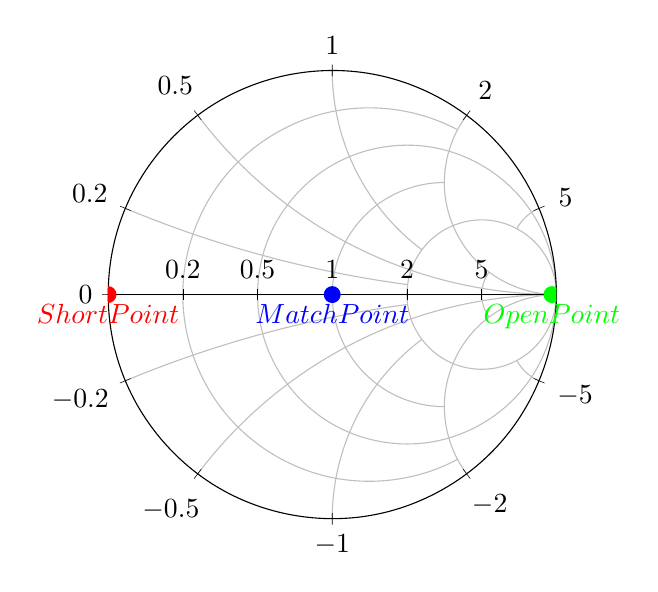
\begin{tikzpicture}
    \begin{smithchart}
      \coordinate (a) at (0pt,0pt);
      \coordinate (b) at (0,0);
      \coordinate (c) at (100,0);
      %\coordinate [label=above:$2+\mathrm{j}1$] (b) at (2,1);
      
      \path[draw=blue,fill=blue] (1,0) circle (0.1cm);
      \path[draw=red,fill=red] (0,0) circle (0.1cm);
      \path[draw=green,fill=green] (100,0) circle (0.1cm);
      %\path [draw=blue] (H) circle (2.83cm);
      %\path[draw=red] (a) circle (2.83cm);
      %\node [draw=red] at (a) [circle through={(b)}] {};
      %\path[draw=blue] (0.2,0.5) circle (0.75cm);
      %\path[draw=blue,fill=blue] (b) circle (0.05cm);
      %\path[draw=blue] (a) -- (2,1);
      %\draw (a) -- ($ (a) !2.3! (b) $) coordinate (c);
    \end{smithchart}

    \node at (a) [color=blue,anchor=north] {$Match Point$};
    \node at (b) [color=red,anchor=north] {$Short Point$};
    \node at (c) [color=green,anchor=north] {$Open Point$};
    %\node at (c) [anchor=south] {$0.213\lambda$};
  \end{tikzpicture}

  %\begin{tikzpicture}
  %  \draw[help lines] (0,0) grid (3,2);
  %  \node (a) at (2,1.5) {$a$};
  %  \node [draw] at (1,1) [circle through={(a)}] {$c$};
  %\end{tikzpicture}
\end{document}
